%% PhD thesis template
%% School of Computing and Communications, Lancaster University, 

%% Copyright 2020 Andrew Moore and Alistair Baron
%
% This work may be distributed and/or modified under the
% conditions of the LaTeX Project Public License, either version 1.3
% of this license or (at your option) any later version.
% The latest version of this license is in
%   http://www.latex-project.org/lppl.txt
% and version 1.3 or later is part of all distributions of LaTeX
% version 2005/12/01 or later.
%
% This work has the LPPL maintenance status `maintained'.
% 
% The Current Maintainer of this work is Alistair Baron
%
% This work consists of the files main.tex, and the other example tex files referenced within.


%
% Heavily based on the formatting and content of Alistair Baron's thesis (https://eprints.lancs.ac.uk/id/eprint/84887/1/2011Baronphd.pdf), Kelly Widdicks's thesis (https://doi.org/10.17635/lancaster/thesis/951), and Andrew Moore's thesis (https://doi.org/10.17635/lancaster/thesis/1408). The thesis is also somewhat based on the Cambridge thesis template: https://github.com/kks32/phd-thesis-template
%
% This was created by Andrew Moore and Alistair Baron with help from Paul Rayson, and Edward Dearden.
%
% Conforms with Lancaster University MANUAL OF ACADEMIC REGULATIONS AND PROCEDURES (MARP) for POSTGRADUATE RESEARCH. This can be found here: https://www.lancaster.ac.uk/media/lancaster-university/content-assets/documents/student-based-services/asq/marp/PGR-Regs.pdf
% For layout information the most relevant pages of that document are Appendix 2.

% This template was updated in November 2022, to apply changes to the regulations made in July 2021.

% Please check that your thesis complies with the current regulations.

% If you have any useful updates for this template, which you think will benefit others, please make these available via github (https://github.com/InfoLab21/scc-thesis-template).


\documentclass[twoside,12pt, a4paper]{report}

% The following sets the whole document to 1.5 line spacing. The line spacing should be 1.5 according to the MARP regulations (Appendix 2), for the purpose of examiner annotation. However, some have a preference for different line spacing (e.g. single). Comment this line out for single line spacing.
\linespread{1.5}

\usepackage[paper=a4paper]{geometry}
\usepackage[utf8]{inputenc}
\usepackage{graphicx}
\usepackage{svg}
\usepackage{hyperref}
\hypersetup{
    colorlinks=false,
    breaklinks=true
}
% All sections and sub sections have to be labelled in the table of contents and thesis. This does this down to the level of subsubsection.
\setcounter{secnumdepth}{4}
\setcounter{tocdepth}{4}

%discourages hyphenated words at end of lines
\hyphenpenalty=5000
\tolerance=1000


% biblography formatting
% NOTE: At the moment both URL and DOI will be displayed, if you have a bib entry that has both URL and DOI please remove the URL so that only one link is displayed, in this case to the DOI. 
\usepackage[style=authoryear,backend=biber,url=true, doi=true, sorting=nyt, natbib=true]{biblatex}
\usepackage{bibentry}
\addbibresource{ref.bib}

% Appendix formatting
\usepackage[title, titletoc]{appendix}
\renewcommand{\appendixpagename}{Appendix}


% for the title page
\usepackage{datetime}
\newdateformat{monthyeardate}{%
  \monthname[\THEMONTH], \THEYEAR}
% For the declaration
% NOTE IF NOT USING OVERLEAF PLEASE REMOVE THIS AND ADD THE WORD COUNT MANUALLY. The software overleaf uses is this: https://app.uio.no/ifi/texcount/
% This has come from overleaf and has been slightly adapted. This counts everything including footnotes and captions I believe and the appendix, but not bibliography.
% https://www.overleaf.com/learn/how-to/Is_there_a_way_to_run_a_word_count_that_doesn%27t_include_LaTeX_commands%3F
\newcommand{\quickwordcount}[1]{%
  \immediate\write18{texcount -0 -sum -merge  #1.tex > #1-words.sum }%
  \input{#1-words.sum}%
}
%
% TO BE FILLED IN
%
\newcommand\thesistitle{The moths of extinction will eat my brain as they will my clothing, and it will all disappear.}
\newcommand\authorname{Alina (Isobel) Hagan} % Full name
\newcommand\authordegrees{MSc} % This does not have to be filled in, but the regulations state that you should include any degrees you have.

\newgeometry{left=35mm, right=25mm, top=25mm, bottom=25mm, asymmetric, includeheadfoot} % This has to come before the header and footer information

% HEADER AND FOOTER STYLE
% https://en.wikibooks.org/wiki/LaTeX/Customizing_Page_Headers_and_Footers
\usepackage{fancyhdr}
% This needs to be smaller or larger depending on your largest header, at the moment we have set it to 15
% even though it states a warning in the latex, as your largest header is most likely 
% not to be a multiline header, but remember this may changed so checks the latex 
% warning for:
% (fancyhdr)                \setlength{\headheight}
% Where it will tell you what to change this too.
\setlength{\headheight}{15pt} 
% For preamble
\fancypagestyle{preamble}{ %
  \fancyhf{} % remove everything
  \fancyfoot[C]{\thepage}
  \renewcommand{\headrulewidth}{0pt} % remove lines as well
  \renewcommand{\footrulewidth}{0pt}
}
\pagestyle{preamble}

% For the main pages
\fancypagestyle{main}{
  \fancyhf{}
  %\fancyhead[R]{\thepage}
  \fancyfoot[C]{\thepage}
  \fancyhead[LE]{\textit{ \nouppercase{\leftmark}} }
  \fancyhead[RO]{\textit{ \nouppercase{\rightmark}} }
  \renewcommand{\headrulewidth}{1pt} % remove lines as well
  \renewcommand{\footrulewidth}{0pt}
}

% For title and chapter pages
\fancypagestyle{plain}{ %
  \fancyhf{} % remove everything
  \fancyfoot[C]{\thepage} %should keep page number
  \renewcommand{\headrulewidth}{0pt} % remove lines as well
  \renewcommand{\footrulewidth}{0pt}
}

% Highlighting your own name in the publication.tex section
\usepackage{xpatch}% or use http://tex.stackexchange.com/a/40705
\makeatletter
\newbibmacro*{name:bold}[2]{%
  \edef\blx@tmp@name{\expandonce#1, \expandonce#2}%
  \def\do##1{\ifdefstring{\blx@tmp@name}{##1}{\bfseries\listbreak}{}}%
  \dolistloop{\boldnames}}
\newcommand*{\boldnames}{}
\makeatother
\xpretobibmacro{name:family}{\begingroup\usebibmacro{name:bold}{#1}{#2}}{}{}
\xpretobibmacro{name:given-family}{\begingroup\usebibmacro{name:bold}{#1}{#2}}{}{}
\xpretobibmacro{name:family-given}{\begingroup\usebibmacro{name:bold}{#1}{#2}}{}{}
\xpretobibmacro{name:delim}{\begingroup\normalfont}{}{}

\xapptobibmacro{name:family}{\endgroup}{}{}
\xapptobibmacro{name:given-family}{\endgroup}{}{}
\xapptobibmacro{name:family-given}{\endgroup}{}{}
\xapptobibmacro{name:delim}{\endgroup}{}{}

\usepackage{lipsum} % just to add random text as an example

%
%


\begin{document}
\pagenumbering{roman}



\begin{titlepage}

\center

\includesvg[scale=0.6]{figures/lu-logo.svg}\vspace{1cm} % This logo was taken from the main Lancaster University website https://www.lancaster.ac.uk/ The same logo can be found, that is not publicly available, in EPS format: https://www.lancaster.ac.uk/current-staff/communications-and-marketing/marketing/resources/#d.en.417655

\huge  \textbf{\thesistitle}

\vspace{2cm}

\Large \textbf{\authorname, \authordegrees}

Department of Physics

Lancaster University

\vfill

\large

A thesis submitted for the degree of

\textit{Doctor of Philosophy}

\vspace{0.5cm}

\monthyeardate\today

\end{titlepage}


%I dedicate this thesis to someone. \textbf{(this is not required when submitting your thesis before your viva and you can add a dedication in your final thesis after your viva if you wish.)}

\clearpage

\begin{center}
\textbf{\thesistitle}

\authorname, \authordegrees.

Department of Physics, Lancaster University

A thesis submitted for the degree of \textit{Doctor of Philosophy}. \monthyeardate\today.
\end{center}

\section*{\centering Abstract}

\textbf{This is the beginning of the abstract that according to the regulations should not be any longer than 300 words. See point 9 in appendix 2 of the regulations \url{https://bit.ly/2Q4H43I}.}


\clearpage

\input{acknowledgements}

\clearpage

\input{declaration}

\clearpage

\input{publications}

\clearpage

\tableofcontents

\clearpage

\listoftables

\clearpage

\listoffigures

\clearpage


\pagestyle{main}
\pagenumbering{arabic}

\chapter{Introduction}
\section{Introduction}
%%Start of your introduction, with a reference to the relevant appendix \ref{appendix_introduction}. Example of different citation styles \citep{moore-rayson-2018-bringing}, and \citet{moore-rayson-2018-bringing}. Example of a table \ref{table:introduction}:
%%\input{tables/introduction/intro_table}
%%\lipsum[2-10]


\chapter{The ATLAS Experiment and The Large Hadron Collider}

\section{Accelerators and Detectors: Basic Principles}
%%\begin{itemize}
%%    \item from the start; Magnetic rigidity(?)
%%    \item acceleration
%%    \item magnetic focussing, FODO, dipole, quadropole
%%    \item detector basics, (relevant) detector types, basic of bethe bloch
%%    \item luminosity calculations, bunch and crossings
%%    \item cross section
%%    \item Limiting factors
%%\end{itemize}


\section{The Large Hadron Collider}
The Large Hadron Collider (LHC) is a modern proton-proton synchrotron located at the CERN complex, outside of Meyrin, Switzerland. At a circumference of approximately 27km the LHC is currently the largest particle accelerator on the planet, and similarly produces the highest centre-of-mass energies for pp collisions, reaching $\sqrt{s}=13\text{TeV}$. The LHC was constructed from 1998-2008 in the tunnel previously occupied by the Large Electron-Positron Collider (LEP). It extends from from the CERN site, across the French border towards the Jura Mountains and round returning through Geneve and Meyrin. It is positioned on a plane inclined at $1.41\%$ between 45-175 metres underground, a measure to protect both the experimental recordings from a large fraction of cosmic ray interference and the surface from any hazardous emissions from either the particle collisions or the synchrotron radiation.

The LHC is supported by a number of smaller accelerator systems designed to provide proton bunches of the correct spacing and energy, these are visible in figure \ref{fig:accel_complex}. The acceleration process begins with the injection of Hydrogen anions ($\text{H}^{-}$) into LINAC\footnote{This was LINAC 2 until 2020, reaching $50\text{MeV}$. During Long Shutdown 2 (LS2) this was obsolesced by LINAC 4}, which provides an acceleration to energies of $160\text{MeV}$ before the beam is passed on the Proton Synchrotron Booster (PSB)\footnote{\href{https://cds.cern.ch/journal/CERNBulletin/2016/32/News\%20Articles/2201549?ln=en}{idk psb}}. This continuous beam from LINAC is stripped of electrons and split consecutively amongst the four PSB rings, accelerated to $1.4\text{GeV}$, and injected into the Proton Synchrotron (PS). PS produces bunches spaced by $25\text{ns}$, accelerates these to $25\text{GeV}$, and passes them over to the Super Proton Synchrotron (SPS) for the final energy increase up to $450\text{GeV}$.


% https://physics.stackexchange.com/questions/474122/how-is-a-proton-beam-separated-into-bunches-in-a-particle-accelerator
%%https://cds.cern.ch/record/446600/
%% "we must make sure that the particle always sees an accelerating voltage at the gap, so the RF frequency must always be an integer multiple (h) of the revolution frequency."
%% https://www.lhc-closer.es/taking_a_closer_look_at_lhc/0.buckets_and_bunches
%% https://home.cern/science/accelerators


%%SPS, LHC, fills reaching an energy of 13.6TeV, 6.8TeV per beam
%%
%%Accelerated by RF Cavities oscillating at 400MHz
%%
%%
%%The LHC 'ring'
%%
%%Dual-core beampipe, common cryostat
%%1232 dipoles, Niobium-titanite construction, ~8.3T at 1.9K
%%474 Quadropoles
%%
%%The Focussing process is performed 



%Points to make
%\begin{itemize}
%    \item precise location
%    \item geometry, straight and curved sections 
%    \item points and active experiments
%    \item full accelerator complex rundown, energies, etc
%    \item run details peak luminosities
%    \item upgrades and futures
%    \item effects of high energies, pileup, etc
%    \item bunch details, bunch grouping, injection etc
%    \item cosmics and radiation protection
%\end{itemize}

\begin{figure}[!h]
    \centering
    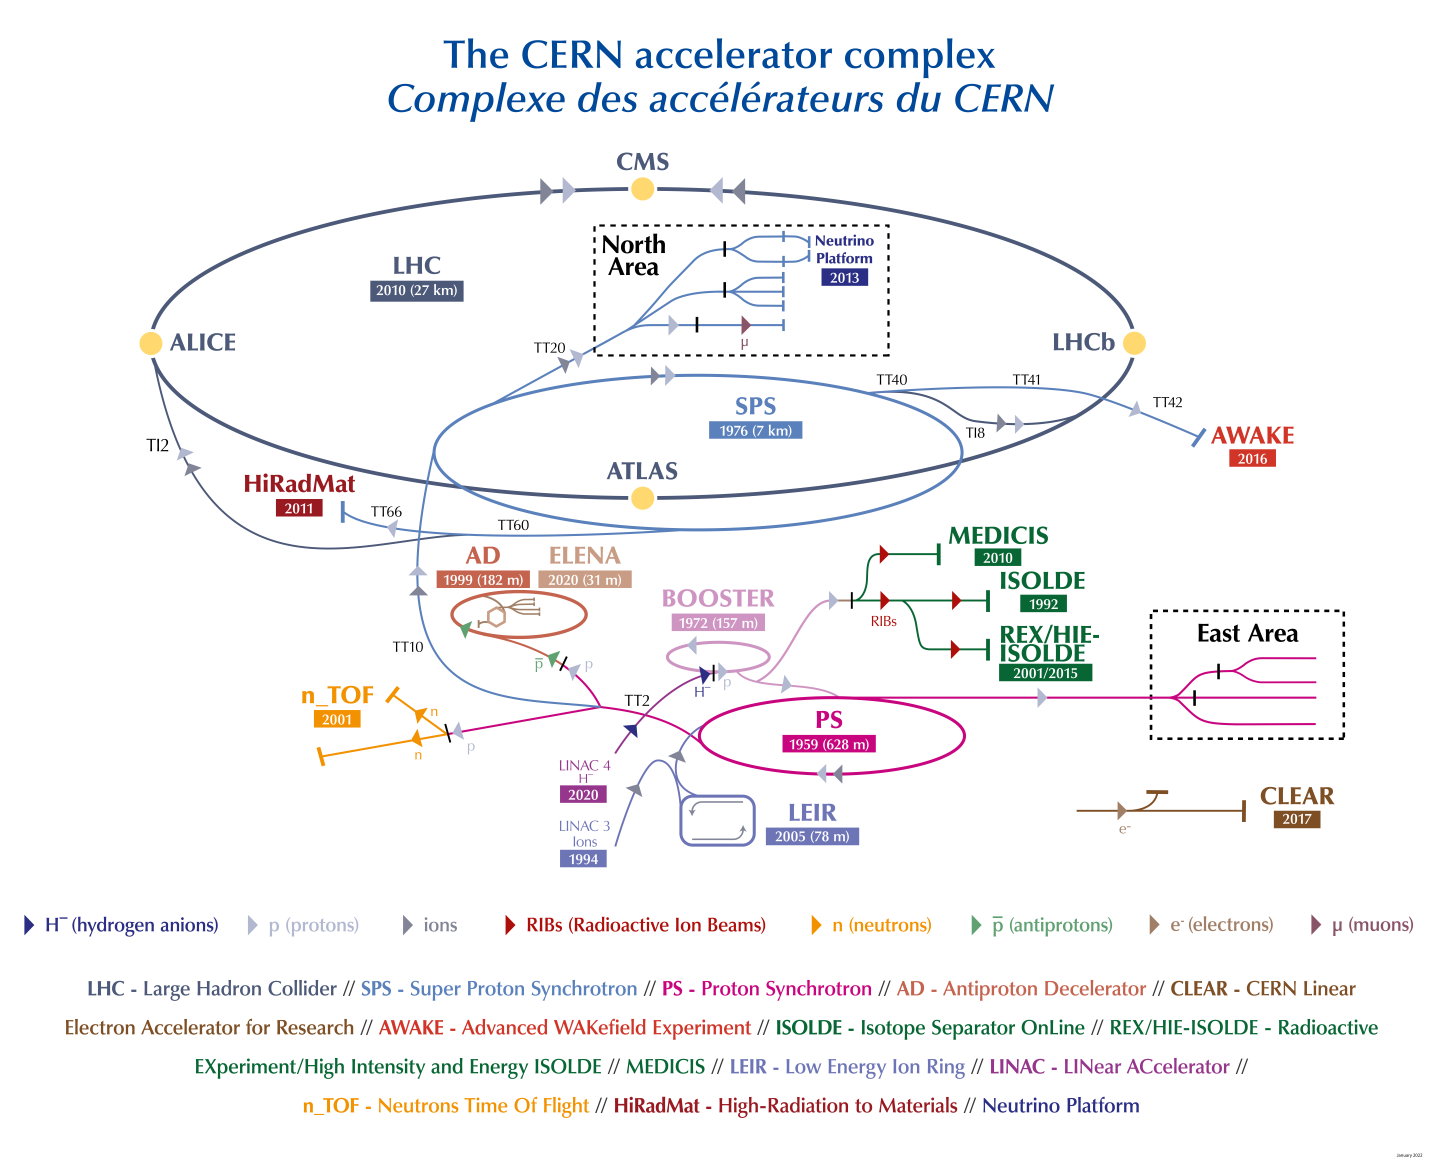
\includegraphics[]{figures/lhc_and_atlas/CCC-v2022.png}
    \caption{CERN Accelerator Complex schematic \cite{Lopienska:2800984}. }
    \label{fig:accel_complex}
\end{figure}




\section{The ATLAS Detector}
\subsection{Overview}
The ATLAS Detector[CITATION] as a general-purpose detector with cylindrical geometry and a forwards-backwards symmetry. It has nearly complete coverage, approaching $4\pi$, in solid angle around the interaction point (IP) which is located centrally within the detector layout.
%%\begin{itemize}
%%    \item Basic detector details.
%%    \item Some collaboration details.
%%    \item Location and control room.
%%    \item Sides.
%%    \item Support infrastructure.
%%\end{itemize}


\subsection{Coordinate system and common variables}
%%\begin{itemize}
%%    \item Rapidity
%%    \item Pseudorapidity
%%    \item Azimuthal angle
%%    \item eta-phi space
%%    \item impact parameters
%%    \item Other varibles required for track definition
%%    \item Common kinematic and analysis variables
%%\end{itemize}

%%\subsection{Inner Detector}
%%\begin{itemize}
%%    \item IBL
%%    \item SCT
%%    \item Pixel
%%    \item Transition Radiation Tracker
%%\end{itemize}
%%\subsection{Calorimetry}
%%\subsubsection{LAr Calormiter}
%%\subsubsection{Hadronic Calorimeter}
%%\subsubsection{Endcap}
%%\subsection{Muon Systems}
%%\begin{itemize}
%%    \item I don't even know yet
%%\end{itemize}
%%\subsection{Magnetic Setup}
%%\begin{itemize}
%%    \item The central solenoidal magnet
%%    \item The toroidal magnets
%%    \item Magnetic diagram
%%\end{itemize}
%%
%%\subsection{Trigger and Data Acquisition}
%%\begin{itemize}
%%    \item L1 and HLT etc
%%    \item Online trigger system - CTP etc
%%    \item offline reprocessing
%%\end{itemize}


\chapter{BLS Trigger; Validation and Purity}

\chapter{Transverse Momentum Dependent Parton Distribution Functions and Quarkonium Production}
%% two sections; theory and statistisc

\chapter{Extraction of TMDs}

\chapter{Conclusions}
\section{Results}
%%Example of a figure \ref{fig:conclusion}:
%%\begin{figure}[!h]
%%    \centering
%%    \includegraphics[scale=0.8]{figures/conclusion/ucrel_logo.png}
%%    \caption{UCREL logo.}
%%    \label{fig:conclusion}
%%\end{figure}


\begin{appendices}

\chapter{Introduction}
\label{appendix_introduction}
\section{Introduction}
%%Start of your introduction, with a reference to the relevant appendix \ref{appendix_introduction}. Example of different citation styles \citep{moore-rayson-2018-bringing}, and \citet{moore-rayson-2018-bringing}. Example of a table \ref{table:introduction}:
%%\input{tables/introduction/intro_table}
%%\lipsum[2-10]


\end{appendices}

\clearpage % Required to make sure the references table of contents page number is correct.
\printbibliography[heading=bibintoc,title=References]

\end{document}

